% !TeX root = presentation.tex
% !TeX spellcheck = en_GB
% !TeX encoding = UTF-8


\documentclass[utf8,t,xcolor=svgnames]{beamer}

\usepackage{beamerthemeblackboard}

%\usepackage{fontspec}
%\setbeamerfont{KGTenThousandReasons}{}
%\setmainfont{KGTenThousandReasons}
%\setromanfont{KGTenThousandReasons}
%\setsansfont{KGTenThousandReasons}
%\setmonofont{KGTenThousandReasons}


\begin{document}

% set handwritten font, necessary packages are loaded in beamerthemeblackboard.sty
%\ECFAugie

\title{Pricing exotic path-dependent options}
\subtitle{The Singular Points method}
\date[2015-10-23]{23\textsuperscript{rd} October, 2015}
\institute[MathMods]{MathMods\\{\small Università degli Studi dell'Aquila}}
%\author[Sudip Sinha]{Sudip Sinha\\{\small Supervisor: Prof. Fabio Antonelli}}
\author{
	\begin{minipage}[t]{0.4\textwidth}
		\begin{center}
			{\small \emph{Candidate:}}\\
			{\textbf{\textsc{Sudip Sinha}}}\\
			{\small Matricola: 228435}
		\end{center}
	\end{minipage}
	\begin{minipage}[t]{0.5\textwidth}
		\begin{center}
			\emph{Supervisor:} \\
			\textsc{Prof. \textbf{Fabio Antonelli}}
		\end{center}
	\end{minipage}
	}


\begin{frame}[plain]
	\maketitle
\end{frame}

\begin{frame}
	\frametitle{Outline}
	\tableofcontents
\end{frame}


\section{Motivation}
\begin{frame}{Introduction}
	\begin{itemize}
		
		\item Assets
		\begin{itemize}
			\item basic assets
			\begin{description}
				\item[riskless] deterministic: $ S_t^0 = e^{rt} $
				\item[risky] stochastic process: $ (S_t)_t $
			\end{description}
			\item derivatives -- contracts on other assets
			\begin{description}
				\item[futures \& forwards] symmetric risk
				\item[options] asymmetric risk
			\end{description}			
		\end{itemize}
		
		\item Problem: pricing derivatives -- finding a fair price
		
		\item Assumptions
		\begin{itemize}
			\item viable / no arbitrage / no free lunch
			\item frictionless
			\item infinitely divisible assets
		\end{itemize}
	\end{itemize}
	
\end{frame}


\begin{frame}{Option types}
	\begin{itemize}
		\item Simple options -- classification of the basis of:
		\begin{description}
			\item[exercise time] European or American
			\item[right of owner] call or put
		\end{description}
		\begin{example}[European call]
			payoff function: $ (S_T - K)_+ = \max \{S_T - K, 0\} $, exercise only at maturity
		\end{example}
		\item Exotic options
		\begin{description}
			\item[\alert{Asian}] payoff: function of average of the underlying
			\item[lookback] payoff: function of extrema of the underlying
			\item[\alert{cliquet, ratchet}] A series of globally or locally, capped or floored, at-the-money options, but where the total premium is determined in advance.
			\item[digital] existence depends on pre-set barriers
		\end{description}
	\end{itemize}
\end{frame}


%	notes: recombinant; n = 3; same outcome; two different paths => different averages
\begin{frame}{Visual representation of risky asset}
	\begin{figure}
		\begin{tikzpicture}
		\matrix[column sep=8mm,row sep=0.4mm,ampersand replacement=\&] (tree){
			\node[header] (t0) {$ t = 0 $};  \&  \node[header] (t1) {$ t = 1 $};  \&  \node[header] (t2) {$ t = 2 $};  \&  \node[header] (t3) {$ t = 3 $};  \\
			\&  \&  \& \node[term] (u3) {$ N_{3,3} \blacktriangleright S_0 u^3 $};  \\
			\&  \&  \node[nterm] (u2) {$ N_{2,2} \blacktriangleright S_0 u^2 $};  \&  \\
			\&  \node[nterm] (u) {$ N_{1,1} \blacktriangleright S_0 u $};  \&  \&  \node[term] (u2d) {$ N_{3,2} \blacktriangleright S_0 u^2 d $};  \\
			\node[term] (s) {$ N_{0,0} \blacktriangleright S_0 $};  \&  \&  \node[nterm] (ud) {$ N_{2,1} \blacktriangleright S_0 u d $};  \&  \\
			\&  \node[nterm] (d) {$ N_{1,0} \blacktriangleright S_0 d $};  \&  \&	\node[term] (ud2) {$ N_{3,1} \blacktriangleright S_0 u d^2 $};  \\
			\&  \&  \node[nterm] (d2) {$ N_{2,0} \blacktriangleright S_0 d^2 $};  \&  \\
			\&  \&  \& \node[term] (d3) {$ N_{3,0} \blacktriangleright S_0 d^3 $};  \\
		};
		
		% Lines out of s
		\draw[->,Yellow,ultra thick] (s) -- (u) node[midway,above,sloped] {$p_u$};
		\draw[->,SpringGreen,ultra thick] (s) -- (d) node[midway,below,sloped] {$p_d$};
		% Lines out of u
		\draw[->,Yellow,ultra thick] (u) -- (u2) node[midway,above,sloped] {$p_u$};
		\draw[->,Moccasin] (u) -- (ud) node[midway,above,sloped] {$p_d$};
		% Lines out of d
		\draw[->,SpringGreen,ultra thick] (d) -- (ud) node[midway,below,sloped] {$p_u$};
		\draw[->,Moccasin] (d) -- (d2) node[midway,below,sloped] {$p_d$};
		% Lines out of u2
		\draw[->,Moccasin] (u2) -- (u3) node[midway,above,sloped] {$p_u$};
		\draw[->,Yellow,ultra thick] (u2) -- (u2d) node[midway,above,sloped] {$p_d$};
		% Lines out of ud
		\draw[->,SpringGreen,ultra thick] (ud) -- (u2d) node[midway,above,sloped] {$p_u$};
		\draw[->,Moccasin] (ud) -- (ud2) node[midway,below,sloped] {$p_d$};
		% Lines out of d2
		\draw[->,Moccasin] (d2) -- (ud2) node[midway,below,sloped] {$p_u$};
		\draw[->,Moccasin] (d2) -- (d3) node[midway,below,sloped] {$p_d$};
		\end{tikzpicture}
		
		%		\caption{A 3-step recombinant tree}
		%		\label{fig:paths}
	\end{figure}
\end{frame}


\begin{frame}{Market models -- discrete vs continuous}
	\begin{tabular}{lll}
		\toprule
		Parameter  &  Discrete  &  Continuous  \\
		\midrule
		Example  &  \cite{Cox1979}  &  \cite{Black1973}  \\
		Theoretical complexity  &  Easy  &  Hard  \\
		Ease of implementation  &  Hard  &  Easy  \\
		Closed-form formula  &  No\footnotemark  &  Yes  \\
		Computational complexity  &  Hard: $ O(2^n) $\footnotemark[1]  &  Easy: $ O(1) $  \\
		Universality  &  Yes  &  No  \\
		\bottomrule
	\end{tabular}
	\footnotetext{CRR: backward recursive}
	
	\begin{theorem}[Convergence in distribution of CRR to BS]
		CRR $ \xrightarrow{d} BS $
	\end{theorem}
	
	\alert{Quest}: Find algorithms with reduced computational complexity under discrete models converging to continuous ones.
\end{frame}

\section{Asian options}

\begin{frame}{Asian options}{Introduction}
	\begin{definition}[Asian options]
		Payoff is a function of some form of averaging on the underlying's price.
	\end{definition}
	
	\begin{example}[fixed-strike Asian call of European type]
		A fixed-strike Asian call of European type, with a strike-price $ K $ would imply that the payoff at maturity is given by $ (A_T - K)_+ $, and the owner of the option may only exercise it at maturity.
	\end{example}
	
	\begin{tabular}{lll}
		\toprule
		Average  &  Discrete  &  Continuous  \\
		\midrule
		AM (arithmetic mean)  &  $ A_n = \frac{1}{n+1} \sum_{i=0}^{n} S_n $  &  $ A_T = \frac{1}{T} \int_{0}^{T} S_t \dif t $  \\
		GM (geometric mean)  &  $ G_n = \left( \prod_{i=0}^{n} S_n \right)^{\frac{1}{n+1}} $  &  $  
		G_T = \exp \left(  \frac{1}{T} \int_{0}^{T} \log(S_t) \dif t  \right) $  \\
		\bottomrule
	\end{tabular}
	
\end{frame}


\begin{frame}{Asian option}{Pre-existing methods}
	\begin{block}{Arithmetic mean}
		\begin{tabular}{cccl}
			\toprule
			Method  &  Type  &  Complexity  &  Remarks  \\
			\midrule
			\cite{Cox1979}  &  Tree  &  $ O(2^n) $  &  simple, accurate, guaranteed convergence  \\
			\cite{Hull1993}  &  Tree  &  $ O(n^3) $  &  accuracy and convergence problems  \\
			\cite{Barraquand1996}  &  Tree  &  $ O(n^3) $  &  accuracy and convergence problems  \\
			\cite{Chalasani1999}  &  Tree  &  $ O(n^4) $  &  thin bounds, but very large memory  \\
			\cite{Vecer2001}  &  PDE  &  $ O(n^2) $  &  not universally applicable  \\
			\cite{dHalluin2005}  &  PDE  &    &  more general than \cite{Vecer2001} \\
			\bottomrule
		\end{tabular}
	\end{block}
	
	\begin{block}{Geometric mean}
		Closed-form formula exist under BS.
	\end{block}
\end{frame}


\begin{frame}{Singular points method for Asian options: introduction}
	Idea: At any node $ N_{i,j} $:
	\begin{itemize}
		\item payoff $ P $: continuous, convex function of the underlying's average $ A $
		\item number of possible averages = number of paths to $ N_{i,j} $ = $ \binom{i}{j} $
		\item these averages completely characterise the payoff; no other payoff being possible under the given tree
		\item the above points $ ((A_{i,j}^l, P_{i,j}^l))_l $ are called \alert{singular points}
		\item payoff is represented as continuous, convex, and piecewise-linear function of the underlying's possible averages, found by joining the singular points
		\item minimum possible average $ A_{i,j}^{\min} = \frac{S_0}{i+1} \left( \frac{1 - d^{i-j+1}}{1-d} + d^{i-j} u \frac{1 - u^{j}}{1-u} \right)$
		\item maximum possible average $ A_{i,j}^{\max} = \frac{S_0}{i+1} \left( \frac{1 - u^{j+1}}{1-u} + u^{j} d \frac{1 - d^{i-j-1}}{1-d} \right) $
	\end{itemize}
\end{frame}


%\begin{frame}{Singular points method: representation of payoff function}
%	\begin{figure}
%		\definecolor{ffffqq}{rgb}{1.,1.,0.}
%		\definecolor{bcduew}{rgb}{0.7372549019607844,0.8313725490196079,0.9019607843137255}
%		\definecolor{zzffff}{rgb}{0.6,1.,1.}
%		\definecolor{ffffff}{rgb}{1.,1.,1.}
%		\begin{tikzpicture}[line cap=round,line join=round,>=triangle 45,x=0.7cm,y=0.6cm]
%		\draw[->,color=ffffff] (-0.5,0.) -- (14.,0.);
%		\foreach \x in {,2.,4.,6.,8.,10.,12.}
%		\draw[shift={(\x,0)},color=ffffff] (0pt,2pt) -- (0pt,-2pt);
%		\draw[color=ffffff] (13.574999979452262,0.09412053045655332) node [anchor=south west] { A};
%		\draw[->,color=ffffff] (0.,-0.5) -- (0.,10.);
%		\foreach \y in {,2.,4.,6.,8.}
%		\draw[shift={(0,\y)},color=ffffff] (2pt,0pt) -- (-2pt,0pt);
%		\draw[color=ffffff] (0.117650656564035,9.563062782941712) node [anchor=west] { P};
%		\clip(-0.5,-0.5) rectangle (14.,10.);
%		\draw [shift={(0.,16.)},line width=1.2pt,dash pattern=on 1pt off 1pt,color=bcduew]  plot[domain=4.71238898038469:5.815035148170625,variable=\t]({1.*15.*cos(\t r)+0.*15.*sin(\t r)},{0.*15.*cos(\t r)+1.*15.*sin(\t r)});
%		\draw [line width=1.2pt,color=ffffqq] (0.,1.)-- (3.9661594381635714,1.5338471143477115);
%		\draw [line width=1.2pt,color=ffffqq] (3.9661594381635714,1.5338471143477115)-- (7.996200825854044,3.309027919319533);
%		\draw [line width=1.2pt,color=ffffqq] (7.996200825854044,3.309027919319533)-- (11.245121140161649,6.072903216796487);
%		\draw [line width=1.2pt,color=ffffqq] (11.245121140161649,6.072903216796487)-- (13.37742288239203,9.235827520930235);
%		\begin{scriptsize}
%		\draw [fill=zzffff] (0.,1.) circle (1.5pt);
%		\draw[color=zzffff] (0.2334155250906906,1.5392875615205421) node {$S_1$};
%		\draw [fill=zzffff] (13.37742288239203,9.235827520930235) circle (1.5pt);
%		\draw[color=zzffff] (13.292638403698577,9.821894241697233) node {$S_5$};
%		\draw[color=bcduew] (11.174926585545943,4.174662414304035) node {continuous price function};
%		\draw [fill=zzffff] (3.9661594381635714,1.5338471143477115) circle (1.5pt);
%		\draw[color=zzffff] (3.8805858785757756,2.080480611645724) node {$S_2$};
%		\draw [fill=zzffff] (7.996200825854044,3.309027919319533) circle (1.5pt);
%		\draw[color=zzffff] (7.92776846437858,3.868770690320237) node {$S_3$};
%		\draw[color=ffffqq] (6.139478484605246,3.2805173749667786) node {discrete price function};
%		\draw [fill=zzffff] (11.245121140161649,6.072903216796487) circle (1.5pt);
%		\draw[color=zzffff] (11.033745797669104,6.715916736630975) node {$S_4$};
%		\end{scriptsize}
%		\end{tikzpicture}
%	\end{figure}
%\end{frame}


\begin{frame}{Singular points method for Asian options}{Start: at maturity ($ i = n $)}
	\begin{minipage}[t]{0.55\linewidth}
		At any node $ N_{n,j} $, three possibilities exist:
		\begin{enumerate}
			\item $ j \in \{ 0, n \} $: end points, only one path possible, only one singular point $ (A, (A-K)_+) $
			\item $ j \notin \{ 0, n \} $ and $ K \in ( A_{n,j}^{\min}, A_{n,j}^{\max} ) $: three singular points:
			\begin{enumerate}
				\item $ ( A_{n,j}^{\min} , 0 ) $
				\item $ ( K , 0 ) $
				\item $ ( A_{n,j}^{\max} , A_{n,j}^{\max} - K ) $
			\end{enumerate}
			\item $ j \notin \{ 0, n \} $ and $ K \notin ( A_{n,j}^{\min}, A_{n,j}^{\max} ) $: two singular points:
			\begin{enumerate}
				\item $ ( A_{n,j}^{\min} , ( A_{n,j}^{\min} - K )_+ ) $
				\item $ ( A_{n,j}^{\max} , ( A_{n,j}^{\max} - K )_+ ) $
			\end{enumerate}
		\end{enumerate}
	\end{minipage}
	\begin{minipage}[t]{0.40\linewidth}
		\begin{itemize}
			\item We discuss only the European case.
			\item The American case needs minor modifications.
		\end{itemize}
		\begin{figure}
			\definecolor{zzffzz}{rgb}{0.6,1.,0.6}
			\definecolor{bfffqq}{rgb}{0.7490196078431373,1.,0.}
			\definecolor{ffffzz}{rgb}{1.,1.,0.6}
			\definecolor{ffffff}{rgb}{1.,1.,1.}
			\begin{tikzpicture}[line cap=round,line join=round,>=triangle 45,x=1.0cm,y=1.0cm]
			\draw[->,color=ffffff] (-0.5,0.) -- (3.5,0.);
			\foreach \x in {,1.,2.,3.}
			\draw[shift={(\x,0)},color=ffffff] (0pt,2pt) -- (0pt,-2pt);
			\draw[color=ffffff] (3.2339019240538707,0.05820970293171456) node [anchor=south west] { A};
			\draw[->,color=ffffff] (0.,-0.5) -- (0.,2.5);
			\foreach \y in {,1.,2.}
			\draw[shift={(0,\y)},color=ffffff] (2pt,0pt) -- (-2pt,0pt);
			\draw[color=ffffff] (0.0727621286646436,2.255161943734117) node [anchor=west] { P};
			\clip(-0.5,-0.5) rectangle (3.5,2.5);
			\draw [line width=2.pt,color=bfffqq] (1.5167156875682812,0.)-- (3.,1.5);
			\draw [line width=0.4pt,dash pattern=on 2pt off 2pt,color=ffffzz] (3.,1.5)-- (3.,0.);
			\draw [line width=2.pt,color=bfffqq] (0.49804588626327045,0.)-- (1.5167156875682812,0.);
			\draw [line width=0.4pt,dash pattern=on 2pt off 2pt,color=ffffzz] (3.,1.5)-- (0.,1.4984358056218274);
			\begin{scriptsize}
			\draw [fill=ffffzz] (1.5167156875682812,0.) circle (2.5pt);
			\draw[color=ffffzz] (1.5167156875682817,-0.3642746881930386) node {$K$};
			\draw [fill=ffffzz] (3.,1.5) circle (2.5pt);
			\draw [fill=ffffzz] (3.,0.) circle (1.5pt);
			\draw[color=ffffzz] (3.0156155380599396,-0.3060649852613241) node {$A_{i,j}^{\max}$};
			\draw [fill=ffffzz] (0.49804588626327045,0.) circle (2.5pt);
			\draw[color=ffffzz] (0.6290177178596299,-0.32061741099425267) node {$A_{i,j}^{\min}$};
			\draw [fill=zzffzz] (0.,1.4984358056218274) circle (2.5pt);
			\draw[color=zzffzz] (0.8618565295864893,1.2510445681620406) node {$\left( A_{i,j}^{\max} - K \right)_+$};
			\end{scriptsize}
			\end{tikzpicture}
			
			\caption{Case 2}
		\end{figure}
		
	\end{minipage}
\end{frame}


\begin{frame}{Singular points method for Asian options}{Up movement at node $ N_{i,j}, \  \forall i < n $}
	\begin{minipage}[t]{0.6\linewidth}
		\begin{enumerate}
			\item Take a singular point $ A_{i+1,j}^l $.
			\item $ B^l = \frac{ ( i+2) A_{i+1,j}^l - S_{i+1,j} }{ i+1 } $.
			\item Each $ B^l \in \left[ A_{i,j}^{\min}, A_{i,j}^{\max} \right] $ is a singular average of $ N_{i,j} $.
			\item For each such $ B^l $, $ B^l_u = \frac{(i+1) B^l + S_{i+1,j+1}}{i+2} $
			\item $ v_{i,j}( B^l ) = \frac{1}{R} \left[ p_u v_{i+1,j+1} \left( B^l_u \right) + p_d v_{i+1,j} \left( A_{i+1,j}^l \right) \right] $.
			\item $ \left( B^l, v_{i,j}( B^l ) \right) $ is a singular point of $ N_{i,j} $.
		\end{enumerate}
	\end{minipage}
	\begin{minipage}[t]{0.3\linewidth}
		\begin{figure}
			\begin{tikzpicture}
			\matrix (tree) [column sep=3em,row sep=1em,ampersand replacement=\&]{
				\node[header] (t0) {$ t = i $};  \&  \node[header] (t1) {$ t = i+1 $}; \\
				\&  \node[term] (u) {$ B^l_u $}; \\
				\node[term] (s) {$ B^l $};  \&  \\
				\&  \node[term] (d) {$ A_{i+1,j}^l $}; \\
			};
			\draw[->,ultra thick] (s) -- (u) node[midway,above,sloped] {Step 2};
			\draw[->,ultra thick] (d) -- (s) node[midway,below,sloped] {Step 1};
			\end{tikzpicture}
		\end{figure}
	\end{minipage}
\end{frame}


\begin{frame}{Singular points method for Asian options}{Down movement at node $ N_{i,j}, \  \forall i < n $}
	\begin{minipage}[t]{0.6\linewidth}
		\begin{enumerate}
			\item Take a singular point $ A_{i+1,j+1}^l $.
			\item $ C^l = \frac{ ( i+2) A_{i+1,j+1}^l - S_{i+1,j+1} }{ i+1 } $.
			\item Each $ C^l \in \left[ A_{i,j}^{\min}, A_{i,j}^{\max} \right] $ is a singular average of $ N_{i,j} $.
			\item For each such $ C^l $, $ C^l_d = \frac{(i+1) C^l + S_{i+1,j}}{i+2}  $
			\item $ v_{i,j}( C^l ) = \frac{1}{R} \left[ p v_{i+1,j+1} \left( A_{i+1,j+1}^l \right) + (1 - p) v_{i+1,j} \left( C^l_d \right) \right] $.
			\item $ \left( C^l, v_{i,j}( C^l ) \right) $ is a singular point of $ N_{i,j} $.
		\end{enumerate}
	\end{minipage}
	\begin{minipage}[t]{0.3\linewidth}
		\begin{figure}
			\begin{tikzpicture}
			\matrix (tree) [column sep=3em,row sep=1em,ampersand replacement=\&]{
				\node[header] (t0) {$ t = i $};  \&  \node[header] (t1) {$ t = i+1 $}; \\
				\&  \node[term] (u) {$ A_{i+1,j+1}^l $}; \\
				\node[term] (s) {$ C^l $};  \&  \\
				\&  \node[term] (d) {$ C^l_d $}; \\
			};
			\draw[->,ultra thick] (u) -- (s) node[midway,above,sloped] {Step 1};
			\draw[->,ultra thick] (s) -- (d) node[midway,below,sloped] {Step 2};
			\end{tikzpicture}
		\end{figure}
	\end{minipage}
\end{frame}


\begin{frame}{Singular points method for Asian options}
	\begin{block}{Aggregation and final price}
		\begin{itemize}
			\item Sort the singular points obtained according to the abscissa.
			\item Repeat the procedure for each node in a backward fashion.
			\item $ P_{0,0}^1 $ is the exact binomial price.
		\end{itemize}
	\end{block}
	\begin{block}{Introduction to approximation}
		\begin{itemize}
			\item Ability to approximate id a key strength of the method.
			\item Not all points necessary $ \implies $ selectively remove points.
			\item Net result: reduction of complexity from exponential time to polynomial time (experimental).
			\item Experimental order of complexity: $ O(n^3) $.
		\end{itemize}
	\end{block}
\end{frame}


\begin{frame}{Singular points method for Asian options: approximations}{Upper estimates}
	\definecolor{ffffqq}{rgb}{1.,1.,0.}
	\definecolor{dqfqcq}{rgb}{0.8156862745098039,0.9411764705882353,0.7529411764705882}
	\definecolor{wqwqwq}{rgb}{0.3764705882352941,0.3764705882352941,0.3764705882352941}
	\definecolor{afeeee}{rgb}{0.6862745098039216,0.9333333333333333,0.9333333333333333}
	\definecolor{ffffff}{rgb}{1.,1.,1.}
	\begin{tikzpicture}[line cap=round,line join=round,>=triangle 45,x=0.59cm,y=0.45cm]
	\draw[->,color=ffffff] (0.,0.) -- (17.,0.);
	\foreach \x in {,2.,4.,6.,8.,10.,12.,14.,16.}
	\draw[shift={(\x,0)},color=ffffff] (0pt,2pt) -- (0pt,-2pt);
	\draw[color=ffffff] (16.503014413215865,0.12712930521358398) node [anchor=south west] { A};
	\draw[->,color=ffffff] (0.,0.) -- (0.,13.);
	\foreach \y in {,2.,4.,6.,8.,10.,12.}
	\draw[shift={(0,\y)},color=ffffff] (2pt,0pt) -- (-2pt,0pt);
	\draw[color=ffffff] (0.158911605284918,12.306834374720044) node [anchor=west] { P};
	\clip(-1.,-1.) rectangle (17.,13.);
	\draw [line width=2.pt,color=afeeee] (16.,12.)-- (12.05,7.25);
	\draw [line width=2.pt,color=afeeee] (8.053489465238158,3.603050081817436)-- (4.,2.5);
	\draw [line width=2.pt,color=afeeee] (4.,2.5)-- (1.,2.);
	\draw [line width=0.4pt,color=wqwqwq] (12.05,7.25)-- (12.,0.);
	\draw [line width=0.4pt,color=wqwqwq] (8.053489465238158,3.603050081817436)-- (8.,0.);
	\draw [line width=0.4pt,color=wqwqwq] (4.,2.5)-- (4.,0.);
	\draw [line width=0.4pt,color=wqwqwq] (1.,2.)-- (1.,0.);
	\draw [line width=2.pt,dash pattern=on 1pt off 1pt on 2pt off 4pt,color=dqfqcq] (4.,2.5)-- (12.05,7.25);
	\draw [line width=0.4pt,color=wqwqwq] (16.,12.)-- (16.,0.);
	\draw [line width=1.2pt,dotted,color=ffffqq] (8.025,4.875)-- (8.053489465238158,3.603050081817436);
	\draw [line width=2.pt,color=afeeee] (8.053489465238158,3.603050081817436)-- (12.05,7.25);
	\draw [color=dqfqcq](2.487010827086094,9.891377575661947) node[anchor=north west] {$f_u(A) \ge f(A) \quad \forall A$};
	\draw [color=ffffqq](2.518793148143078,8.397608239402336) node[anchor=north west] {$(f_u - f)(A) \le \varepsilon \quad \forall A$};
	\begin{scriptsize}
	\draw [fill=afeeee] (16.,12.) circle (2.0pt);
	\draw[color=afeeee] (16.40766745004491,11.512276217135144) node {$S_5$};
	\draw [fill=afeeee] (12.05,7.25) circle (2.0pt);
	\draw[color=afeeee] (12.434877317921963,6.840274250535932) node {$S_4$};
	\draw [fill=afeeee] (8.053489465238158,3.603050081817436) circle (2.0pt);
	\draw[color=afeeee] (8.430304864742027,3.1217420730386003) node {$S_3$};
	\draw [fill=afeeee] (4.,2.5) circle (2.0pt);
	\draw[color=afeeee] (4.362167769448127,2.041142978723137) node {$S_2$};
	\draw[color=afeeee] (6.396236317095077,2.8039188100046406) node {f};
	\draw [fill=afeeee] (1.,2.) circle (2.0pt);
	\draw[color=afeeee] (1.4064119111486517,1.6915373893857808) node {$S_1$};
	\draw [fill=afeeee] (16.,0.) circle (2.0pt);
	\draw[color=afeeee] (16.185191202646024,-0.43787847294175086) node {$A_5$};
	\draw [fill=afeeee] (12.,0.) circle (2.0pt);
	\draw[color=afeeee] (12.117054107352125,-0.4696607992451468) node {$A_4$};
	\draw [fill=afeeee] (8.,0.) circle (2.0pt);
	\draw[color=afeeee] (8.080699333115207,-0.5332254518519388) node {$A_3$};
	\draw [fill=afeeee] (4.,0.) circle (2.0pt);
	\draw[color=afeeee] (4.04434455887829,-0.5650077781553349) node {$A_2$};
	\draw [fill=afeeee] (1.,0.) circle (2.0pt);
	\draw[color=afeeee] (1.056806379521832,-0.5332254518519388) node {$A_1$};
	\draw[color=dqfqcq] (9.002386643767732,6.109280745557824) node {$f_u$};
	\draw [fill=dqfqcq] (8.025,4.875) circle (2.0pt);
	\draw[color=dqfqcq] (7.508617554089503,5.092246303849152) node {$R_3$};
	\draw[color=ffffqq] (8.398522543685043,4.265905819960856) node {$\varepsilon_3$};
	\draw[color=afeeee] (10.464373412388976,5.314722587972924) node {f};
	\end{scriptsize}
	\end{tikzpicture}
\end{frame}


\begin{frame}{Singular points method for Asian options: approximations}{Lower estimates}
	\definecolor{ffffqq}{rgb}{1.,1.,0.}
	\definecolor{wqwqwq}{rgb}{0.3764705882352941,0.3764705882352941,0.3764705882352941}
	\definecolor{afeeee}{rgb}{0.6862745098039216,0.9333333333333333,0.9333333333333333}
	\definecolor{ffffff}{rgb}{1.,1.,1.}
	\begin{tikzpicture}[line cap=round,line join=round,>=triangle 45,x=0.59cm,y=0.45cm]
	\draw[->,color=ffffff] (0.,0.) -- (17.,0.);
	\foreach \x in {,2.,4.,6.,8.,10.,12.,14.,16.}
	\draw[shift={(\x,0)},color=ffffff] (0pt,2pt) -- (0pt,-2pt);
	\draw[color=ffffff] (16.983734759565976,0.15704689406799202) node [anchor=south west] { A};
	\draw[->,color=ffffff] (0.,0.) -- (0.,13.);
	\foreach \y in {,2.,4.,6.,8.,10.,12.}
	\draw[shift={(0,\y)},color=ffffff] (2pt,0pt) -- (-2pt,0pt);
	\draw[color=ffffff] (0.19630858508193877,12.246817877668772) node [anchor=west] { P};
	\clip(-1.,-1.) rectangle (17.,13.);
	\draw [line width=2.pt,color=afeeee] (4.,2.5)-- (12.,8.);
	\draw [line width=2.pt,color=afeeee] (16.,12.)-- (12.,8.);
	\draw [line width=0.4pt,color=wqwqwq] (12.,8.)-- (12.,0.);
	\draw [line width=0.4pt,color=wqwqwq] (4.,2.5)-- (4.,0.);
	\draw [line width=0.4pt,color=wqwqwq] (1.,2.)-- (1.,0.);
	\draw [line width=2.pt,dash pattern=on 2pt off 2pt,color=afeeee] (4.,2.5)-- (7.,3.);
	\draw [line width=2.pt,dash pattern=on 2pt off 2pt,color=afeeee] (12.,8.)-- (7.,3.);
	\draw [line width=0.4pt,color=wqwqwq] (7.,3.)-- (6.998942733420039,0.);
	\draw [line width=0.4pt,color=wqwqwq] (16.,12.)-- (16.,0.);
	\draw [line width=1.2pt,dash pattern=on 1pt off 1pt,color=ffffqq] (7.000519372007349,4.562857068255052)-- (7.,3.);
	\draw [color=afeeee](1.9857588593058553,11.540106854362808) node[anchor=north west] {$f_d(A) \le f(A) \quad \forall A$};
	\draw [color=ffffqq](1.9857588593058553,10.48004031940386) node[anchor=north west] {$(f - f_d) (A) \le \delta  \quad  \forall A$};
	\draw [line width=2.pt,color=afeeee] (1.,2.)-- (4.,2.5);
	\begin{scriptsize}
	\draw [fill=afeeee] (16.,12.) circle (2.0pt);
	\draw[color=afeeee] (16.355547287303775,11.500845130845809) node {$S_4$};
	\draw [fill=afeeee] (12.,8.) circle (2.0pt);
	\draw[color=afeeee] (12.429375585664998,7.260578991010025) node {$S_3$};
	\draw [fill=afeeee] (4.,2.5) circle (2.0pt);
	\draw[color=afeeee] (4.4592470313382835,2.03876976324929) node {$S_2$};
	\draw [fill=afeeee] (1.,2.) circle (2.0pt);
	\draw[color=afeeee] (1.2790479530108758,1.5283673575283159) node {$S_1$};
	\draw [fill=afeeee] (16.,0.) circle (2.0pt);
	\draw[color=afeeee] (16.041453551172673,-0.7095508829405706) node {$A_4$};
	\draw [fill=afeeee] (12.,0.) circle (2.0pt);
	\draw[color=afeeee] (12.076020132517508,-0.6702891594235725) node {$A_3$};
	\draw [fill=afeeee] (4.,0.) circle (2.0pt);
	\draw[color=afeeee] (4.105891578190794,-0.6702891594235725) node {$A_2$};
	\draw [fill=afeeee] (1.,0.) circle (2.0pt);
	\draw[color=afeeee] (1.0042159338961614,-0.7488126064575684) node {$A_1$};
	\draw [fill=afeeee] (6.998942733420039,0.) circle (2.0pt);
	\draw[color=afeeee] (7.011258637403488,-0.7095508829405706) node {$A_{23}$};
	\draw [fill=afeeee] (7.,3.) circle (2.0pt);
	\draw[color=afeeee] (7.482399241600141,2.156554933800284) node {$R_{23}$};
	\draw[color=afeeee] (5.833407126911855,2.156554933800284) node {$f_d$};
	\draw[color=afeeee] (9.798840545567018,4.9441373035071425) node {$f_d$};
	\draw [fill=afeeee] (7.000519372007349,4.562857068255052) circle (2.0pt);
	\draw[color=afeeee] (6.5793797502232225,5.925680391432093) node {$S_{23}$};
	\draw[color=ffffqq] (7.286090656518202,3.7270238744802042) node {$\delta_4$};
	\end{scriptsize}
	\end{tikzpicture}
\end{frame}


\begin{frame}{Singular points method for Asian options: numerical results}
	\begin{tabular}{crcccc}
		\toprule
		&         &  \multicolumn{2}{c}{$ K = 90 $}  &  \multicolumn{2}{c}{$ K = 110 $}  \\
		\cmidrule(lr){3-4}\cmidrule(lr){5-6}
		&  $ n $  &  $ \sigma = 0.2 $  &  $ \sigma = 0.4 $  &  $ \sigma = 0.2 $  &  $ \sigma = 0.4 $  \\
		\midrule
		\multirow{2}{2em}{Bin}
		&   10  &  14.5912  &  17.8033  &  2.5100  &  6.6523  \\
		&   25  &  15.1535  &  18.6786  &  2.6270  &  7.3451  \\
		\midrule
		\multirow{6}{2em}{SP}
		&   10  &  14.5925  &  17.8068  &  2.5090  &  6.6511  \\
		&   25  &  15.1535  &  18.6785  &  2.6270  &  7.3449  \\
		&   50  &  15.3524  &  19.0420  &  2.6673  &  7.4563  \\
		&  100  &  15.4732  &  19.2696  &  2.6886  &  7.5174  \\
		&  200  &  15.5453  &  19.4065  &  2.6996  &  7.5502  \\
		&  400  &  15.5861  &  19.4845  &  2.7053  &  7.5674  \\
		\bottomrule
	\end{tabular}
\end{frame}


\begin{frame}{Singular points method for Asian options: summary}
	\begin{itemize}
		\neu Introduced by Gaudenzi \emph{et al} \cite{Gaudenzi2010} in 2010.
		\pro Convergent to exact CRR and thus BS.
		\pro Approximation -- \emph{A priori} error bounds.
		\pro Fast -- experimental order of complexity $ O(n^3) $.
		\con Difficult to compute theoretical complexity.
		\con Depends on the recombinant nature of the underlying's tree.
		\con<alert@1-> Not extensible to GM, since the price function is non-linear. $ G_u = \left( G^{i+1} S_0 u^{-i+2j+1} \right)^{\frac{1}{i+2}} \propto G^{\frac{i+1}{i+2}} $
		\con<alert@1-> Assumes constant volatility, hence not applicable to local volatility models.
	\end{itemize}
\end{frame}



\section{Cliquet options}

\begin{frame}
	\frametitle{Experimental computational complexity -- $ O(m^2) $}
	
	% This plot was generated by plotly
	\begin{figure}
		\centering
		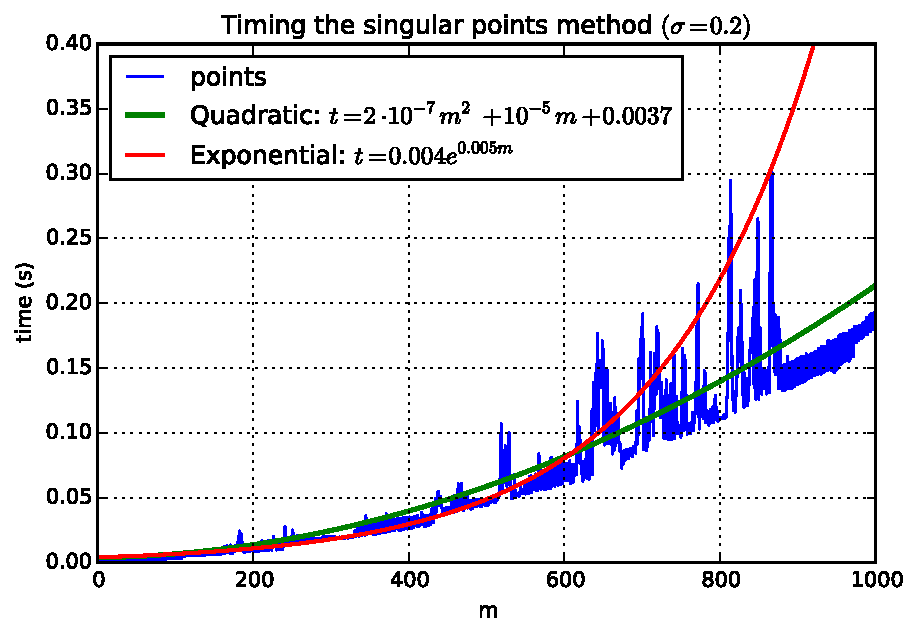
\includegraphics[width=0.85\linewidth]{../img/timing-cliquet}
	\end{figure}
\end{frame}



\section{Final comments}

\begin{frame}{Further research}
\end{frame}


\begin{frame}[plain,c]
	%\frametitle{A first slide}
	
	\begin{center}
		{\Huge Questions?}
	\end{center}
	
	\vfill
	
	\begin{center}
		{\Huge Thank you!}
	\end{center}
	
\end{frame}


\appendix
%\section<presentation>*{\appendixname}
%\subsection<presentation>*{Bibliography}

\begin{frame}[allowframebreaks]
	\frametitle<presentation>{Bibliography}
	\printbibliography
\end{frame}


\end{document}
